\documentclass{article}

% 导入宏包
\usepackage{fancyhdr}
\usepackage{ctex}
\usepackage{listings}
\usepackage{graphicx}
\usepackage[a4paper, body={18cm,22cm}]{geometry}
\usepackage{amsmath,amsthm,amssymb,amstext,wasysym,enumerate,graphicx}
\usepackage{float,abstract,booktabs,indentfirst,amsmath}
\usepackage{array}
\usepackage{multirow}
\usepackage{multicol}
\usepackage{url}
\usepackage{diagbox}
\usepackage{enumitem}
\usepackage{xcolor}
\usepackage{makecell}
\usepackage{tikz}
\usepackage{tcolorbox}
\usetikzlibrary{positioning, arrows.meta}
\usepackage[bookmarks=true, colorlinks, citecolor=blue, linkcolor=black]{hyperref}


% 设置段落
\renewcommand\arraystretch{1.4}
\setlength{\parindent}{2em}
\setCJKmonofont{黑体}

% 设置高亮文字
\newtcbox{\mybox}[1][red]
{on line, arc = 0pt, outer arc = 0pt,
	colback = #1!10!white, colframe = #1!50!black,
	boxsep = 0pt, left = 1pt, right = 1pt, top = 2pt, bottom = 2pt,
	boxrule = 0pt, bottomrule = 1pt, toprule = 1pt}

% 配置代码显示
\lstset{
	xleftmargin = 3em,
	xrightmargin = 3em,
	aboveskip = 1em,
	backgroundcolor = \color{white},
	basicstyle = \small\ttfamily,
	rulesepcolor = \color{gray},
	breaklines = true,
	numbers = left,
	numberstyle = \small,
	numbersep = -14pt,
	keywordstyle = \color{purple}\bfseries,
	commentstyle = \color{green!60!black}, % 修改注释颜色
	stringstyle = \color{red!60!green!90!blue!90},
	morekeywords = {ASSERT, int64_t, uint32_t},
	moreemph = {ASSERT, NULL},
	emphstyle = \color{red}\bfseries,
	moreemph = [2]{int64\_t, uint32\_t, tid\_t, uint8\_t, int16\_t, uint16\_t, int32\_t, size\_t, bool},
	emphstyle = [2]\color{purple}\bfseries,
	frame = shadowbox,
	showspaces = false,
	columns = fixed
	morecomment = [l][\color{green!60!black}]{+}, % 设置以+开头的代码行为绿色
}

%--------------------页眉--------------------%

\pagestyle{fancy}
\fancyhead[L]{}
\fancyhead[R]{}
\fancyhead[C]{华东师范大学软件工程学院实验报告}
\fancyfoot[C]{-\thepage-}
\renewcommand{\headrulewidth}{1.5pt}

%--------------------标题--------------------%

\begin{document}
	\begin{center}
		{\Large{\textbf{\heiti 华东师范大学软件工程学院实验报告}}}
		\begin{table}[htb]
			\flushleft
			\begin{tabular}{p{0.4\linewidth}p{0.27\linewidth}p{0.28\linewidth}}\\
				\textbf{实验课程}:数据库系统及其应用实践  & \textbf{年级}:2023级       & \textbf{实验成绩}:  \\
				\textbf{实验名称}:Lab-05 & \textbf{姓名}:顾翌炜         &                 \\
				\textbf{实验编号}:Lab-05     & \textbf{学号}:10235101527 & \textbf{实验日期}:2025/05/15  \\
				\textbf{指导教师}:姚俊杰     & \textbf{组号}:01            & \textbf{实验时间}:2课时  \\ 
			\end{tabular}
		\end{table}
	\end{center}
	\rule{\textwidth}{2pt}
	
	% 生成目录
	\tableofcontents
	
	\vspace{1cm}
	
	\section{实验目标}
	
	本实验旨在帮助学生深入理解数据库存储结构和索引机制,掌握索引的创建与使用方法,分析存储与索引对数据库性能的影响,提升数据库管理能力。通过实验,学生将能够熟练运用 MySQL 数据库进行存储管理与索引优化,为实际数据库应用开发和管理提供理论与实践基础。
	
	\section{实验要求}
	
	\begin{enumerate}[noitemsep, label={{\arabic*})}]
		\item \textbf{深入探究存储原理}:通过本次实验,学生能够深入了解数据库中数据的物理存储方式,包括数据文件、日志文件等的组织形式。例如,了解关系型数据库中表是如何以页或块的形式存储在磁盘上的,以及这些存储单位如何进行空间分配和管理,从而为后续学习数据库的高效操作奠定基础。
		
		\item \textbf{掌握存储参数配置}:使学生熟悉数据库存储相关的参数配置,如表空间大小、数据块大小等。以 Oracle 数据库为例,学生将学会如何根据实际应用需求合理设置表空间的大小,以及如何调整数据块大小以优化存储空间利用率和数据读写性能,从而更好地管理和维护数据库存储环境。
		
		\item \textbf{创建索引的实践操作}:让学生熟练掌握在数据库中创建不同类型索引(如 B 树索引、哈希索引等)的方法。以 MySQL 数据库为例,学生将学会使用 SQL 语句创建单列索引、组合索引,并理解在什么情况下适合创建哪种类型的索引。例如,在一个包含大量用户信息的表中,如果经常根据用户姓名进行查询,就可以创建一个基于用户姓名列的 B 树索引,以加快查询速度。
		
		\item \textbf{优化查询性能}:使学生能够通过合理使用索引显著提高数据库查询性能。 通过实验,学生将了解到索引是如何帮助数据库管理系统快速定位数据的。例如,在一个大型电商数据库中,对于频繁查询商品价格和库存的场景,通过在价格和库存字段上创建合适的索引,可以大大减少查询时需要扫描的数据量,从而将查询响应时间从数秒缩短到毫秒级别,提升用户体验。
	\end{enumerate}\textbf{}
	
	\section{实验过程记录}
	
	\subsection{启动MySQL数据库}
	
	在数据库管理工具中启动数据库
	
	\subsection{通过PowerShell连接到MySQL}
	
	通过在命令行输入以下指令,通过PowerShell连接到MySQL
	
	\begin{lstlisting}[title=通过PowerShell连接到MySQL, tabsize=4]
	mysql -h localhost -P 3306 -u root -p
	\end{lstlisting}
	
	\begin{figure}[H]
		\centering
		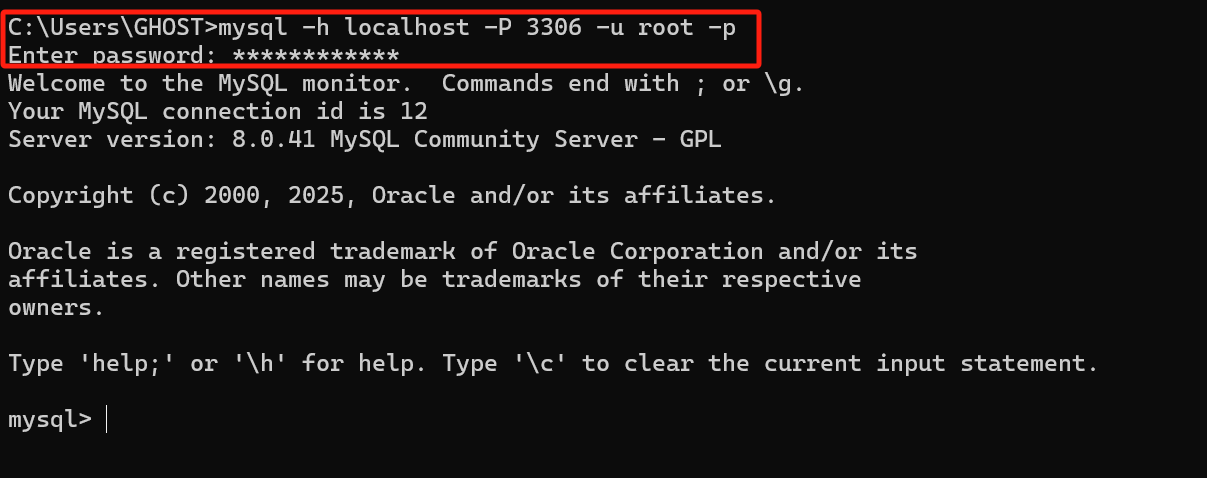
\includegraphics[width=11cm]{./images/1.连接数据库.png}
		\caption{连接数据库}
	\end{figure}
	
	\subsection{执行指定SQL语句}
	
	执行以下SQL语句,创建一个名为mydb的数据库,同时在该模式下创建数据表mytakes和
	mysection
	
	\begin{lstlisting}[language=sql, title=创建db数据库, tabsize=4]
	DROP DATABASE IF EXISTS mydb;
	CREATE DATABASE mydb;
	USE mydb;
	DROP TABLE IF EXISTS mytakes;
	CREATE TABLE `mytakes` (
		`ID` varchar(5) NOT NULL,
		`course_id` varchar(8) NOT NULL,
		`sec_id` varchar(8) NOT NULL,
		`semester` varchar(6) NOT NULL,
		`year` int NOT NULL,
		`grade` varchar(2) DEFAULT NULL,
		PRIMARY KEY (`ID`,`course_id`,`sec_id`,`semester`,`year`) USING BTREE
	);
	insert into mytakes select * from college.takes;
	
	DROP TABLE IF EXISTS mysection;
	CREATE TABLE `mysection` (
		`section_id` int NOT NULL AUTO_INCREMENT,
		`year` int NOT NULL,
		`semester` varchar(6) NOT NULL,
		`building` varchar(15),
		`room_number` varchar(7),
		`time_slot_id` varchar(4),
		`course_id` varchar(8),
		`sec_id` varchar(8) NOT NULL,
		PRIMARY KEY (`section_id`)
	);
	insert into mysection (`course_id`, `sec_id`, `semester`, `year`, `building`, `room_number`, `time_slot_id`)
	select * from college.section;
	\end{lstlisting}
	
	得到以下结果:
	
	\begin{figure}[H]
		\centering
		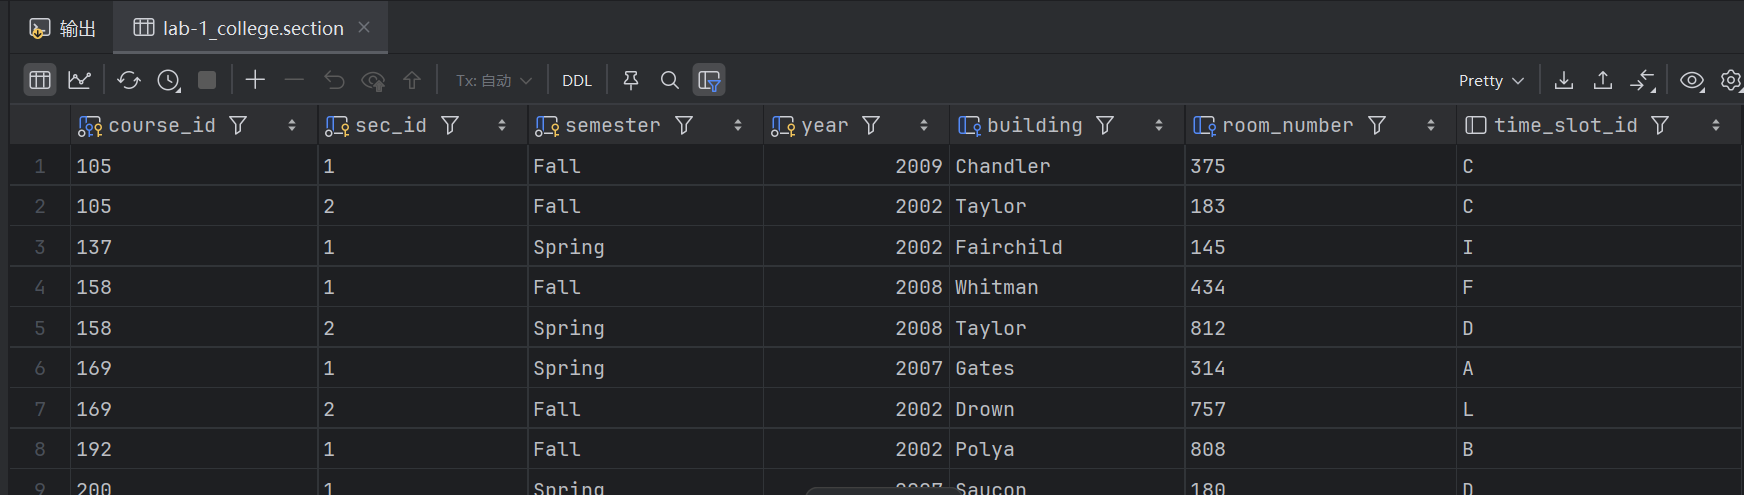
\includegraphics[width=11cm]{./images/2.创建db.png}
		\caption{创建db}
	\end{figure}
	
	创建成功,开始实验
	
	\subsection{观察Insert查询性能}
	
	执行下列语句,观察索引对查询性能的影响,记录每条语句返回的结果并解释其完成的操作
	
	\begin{lstlisting}[language=sql, title=索引对查询性能的影响 - 总, tabsize=4]
	EXPLAIN insert into mytakes select * from `lab-1_college`.takes;
	EXPLAIN ANALYZE insert into mytakes select * from `lab-1_college`.takes;
	EXPLAIN SELECT * FROM mytakes;
	EXPLAIN SELECT * FROM mytakes LIMIT 1;
	EXPLAIN ANALYZE SELECT * FROM mytakes;
	EXPLAIN ANALYZE SELECT * FROM mytakes LIMIT 1;
	\end{lstlisting}
	
	接下来逐行执行,查看每行的结果并分析:
	
	\begin{lstlisting}[language=sql, title=索引对查询性能的影响, tabsize=4]
	USE mydb;
	
	EXPLAIN insert into mytakes select * from college.takes;
	\end{lstlisting}
	
	得到以下结果:
	
	\begin{verbatim}
		+--+-----------+-------+----------+----+-------------+----+-------+----+-----+--------+-----+
		|id|select_type|table  |partitions|type|possible_keys|key |key_len|ref |rows |filtered|Extra|
		+--+-----------+-------+----------+----+-------------+----+-------+----+-----+--------+-----+
		|1 |INSERT     |mytakes|null      |ALL |null         |null|null   |null|null |null    |null |
		|1 |SIMPLE     |takes  |null      |ALL |null         |null|null   |null|27012|100     |null |
		+--+-----------+-------+----------+----+-------------+----+-------+----+-----+--------+-----+
	\end{verbatim}
	
	通过这个执行计划,我们可以看到在插入操作中,MySQL 没有使用索引,而是扫描了整个 college.takes 表。这可能会影响查询性能,特别是在数据量较大的情况下。为了提高性能,可以考虑在 college.takes 表上创建适当的索引。
	
	\begin{lstlisting}[language=sql, title=索引对查询性能的影响, tabsize=4]
	EXPLAIN ANALYZE insert into mytakes select * from college.takes;
	\end{lstlisting}
	
	得到以下结果:
	
	\begin{verbatim}
	+--------------------------------------------------------------------------------------------+
	|EXPLAIN                                                                                     |
	+--------------------------------------------------------------------------------------------+
	|-> Insert into mytakes                                                                      |
	|-> Table scan on takes  (cost=2725 rows=27012) (actual time=2.99..35.4 rows=30000 loops=1)  |
	+--------------------------------------------------------------------------------------------+
	\end{verbatim}
	
	通过这个执行计划,我们可以看到在插入操作中,MySQL 对 college.takes 表进行了全表扫描,估计需要扫描27012行,实际扫描了30000行,执行时间大约在2.99秒到35.4秒之间。这可能会影响查询性能,特别是在数据量较大的情况下。为了提高性能,可以考虑在 college.takes 表上创建适当的索引。
	
	\begin{lstlisting}[language=sql, title=索引对查询性能的影响, tabsize=4]
	EXPLAIN SELECT * FROM mytakes;
	\end{lstlisting}
	
	得到以下结果:
	
	\begin{verbatim}
	+--+-----------+-------+----------+----+-------------+----+-------+----+-----+--------+-----+
	|id|select_type|table  |partitions|type|possible_keys|key |key_len|ref |rows |filtered|Extra|
	+--+-----------+-------+----------+----+-------------+----+-------+----+-----+--------+-----+
	|1 |SIMPLE     |mytakes|null      |ALL |null         |null|null   |null|30000|100     |null |
	+--+-----------+-------+----------+----+-------------+----+-------+----+-----+--------+-----+
	\end{verbatim}
	
	通过这个执行计划,我们可以看到在查询操作中,MySQL 对 mytakes 表进行了全表扫描,估计需要扫描30000行。这可能会影响查询性能,特别是在数据量较大的情况下。为了提高性能,可以考虑在 mytakes 表上创建适当的索引。
	
	\begin{lstlisting}[language=sql, title=索引对查询性能的影响, tabsize=4]
	EXPLAIN SELECT * FROM mytakes LIMIT 1;
	\end{lstlisting}
	
	得到以下结果:
	
	\begin{verbatim}
	+--+-----------+-------+----------+----+-------------+----+-------+----+-----+--------+-----+
	|id|select_type|table  |partitions|type|possible_keys|key |key_len|ref |rows |filtered|Extra|
	+--+-----------+-------+----------+----+-------------+----+-------+----+-----+--------+-----+
	|1 |SIMPLE     |mytakes|null      |ALL |null         |null|null   |null|30000|100     |null |
	+--+-----------+-------+----------+----+-------------+----+-------+----+-----+--------+-----+
	\end{verbatim}
	
	通过这个执行计划,我们可以看到在查询操作中,尽管只返回一行数据,MySQL 仍然对 mytakes 表进行了全表扫描,估计需要扫描30000行。这可能会影响查询性能,特别是在数据量较大的情况下。为了提高性能,可以考虑在 mytakes 表上创建适当的索引。
	
	\begin{lstlisting}[language=sql, title=索引对查询性能的影响, tabsize=4]
	EXPLAIN ANALYZE SELECT * FROM mytakes;
	\end{lstlisting}
	
	得到以下结果:
	
	\begin{verbatim}
	+---------------------------------------------------------------------------------------------+
	|EXPLAIN                                                                                      |
	+---------------------------------------------------------------------------------------------+
	|-> Table scan on mytakes  (cost=3024 rows=30000) (actual time=2.35..13.2 rows=30000 loops=1) |
	+---------------------------------------------------------------------------------------------+
	\end{verbatim}
	
	通过这个执行计划,我们可以看到在查询操作中,MySQL 对 mytakes 表进行了全表扫描,估计需要扫描30000行,实际扫描了30000行,执行时间大约在2.35秒到13.2秒之间。这可能会影响查询性能,特别是在数据量较大的情况下。为了提高性能,可以考虑在 mytakes 表上创建适当的索引。
	
	\begin{lstlisting}[language=sql, title=索引对查询性能的影响, tabsize=4]
	EXPLAIN ANALYZE SELECT * FROM mytakes LIMIT 1;
	\end{lstlisting}
	
	得到以下结果:

	\begin{verbatim}
	+------------------------------------------------------------------------------------------+
	|EXPLAIN                                                                                   |
	+------------------------------------------------------------------------------------------+
	|-> Limit: 1 row(s)  (cost=3024 rows=1) (actual time=0.286..0.286 rows=1 loops=1)          |
	|-> Table scan on mytakes  (cost=3024 rows=30000) (actual time=0.284..0.284 rows=1 loops=1)|
	+------------------------------------------------------------------------------------------+
	\end{verbatim}
	
	通过这个执行计划,我们可以看到在查询操作中,尽管只返回一行数据,MySQL 仍然对 mytakes 表进行了全表扫描,扫描了30000行数据。虽然实际执行时间较短(0.284秒),但这可能会影响查询性能,特别是在数据量较大的情况下。为了提高性能,可以考虑在 mytakes 表上创建适当的索引。
	
	\subsection{观察SELECT with INDEX查询性能}
	
	执行下列语句,观察索引对查询性能的影响,记录每条语句返回的结果并解释其完成的操作
	
	\begin{lstlisting}[language=sql, title=索引对查询性能的影响 - 总, tabsize=4]
	SHOW INDEXES FROM mytakes; -- 执行结果要同上图所示,如有多余的index,请先drop删除掉
	EXPLAIN SELECT * FROM mytakes where course_id='158';
	EXPLAIN ANALYZE SELECT * FROM mytakes where course_id='158';
	CREATE INDEX course_id ON mytakes(course_id);
	EXPLAIN SELECT * FROM mytakes where course_id='158';
	EXPLAIN ANALYZE SELECT * FROM mytakes where course_id='158';
	-- 分析索引失效原因
	EXPLAIN SELECT * FROM mytakes where course_id=158;
	EXPLAIN ANALYZE SELECT * FROM mytakes where course_id=158;
	-- 删除索引
	DROP INDEX course_id ON mytakes;
	\end{lstlisting}
	
	接下来逐行执行,查看每行的结果并分析:
	
	\begin{lstlisting}[language=sql, title=索引对查询性能的影响, tabsize=4]
	USE mydb;
	SHOW INDEXES FROM mytakes; -- 执行结果要同上图所示,如有多余的index,请先drop删除掉
	\end{lstlisting}
	
	得到结果如下图所示:
	
	\begin{figure}[H]
		\centering
		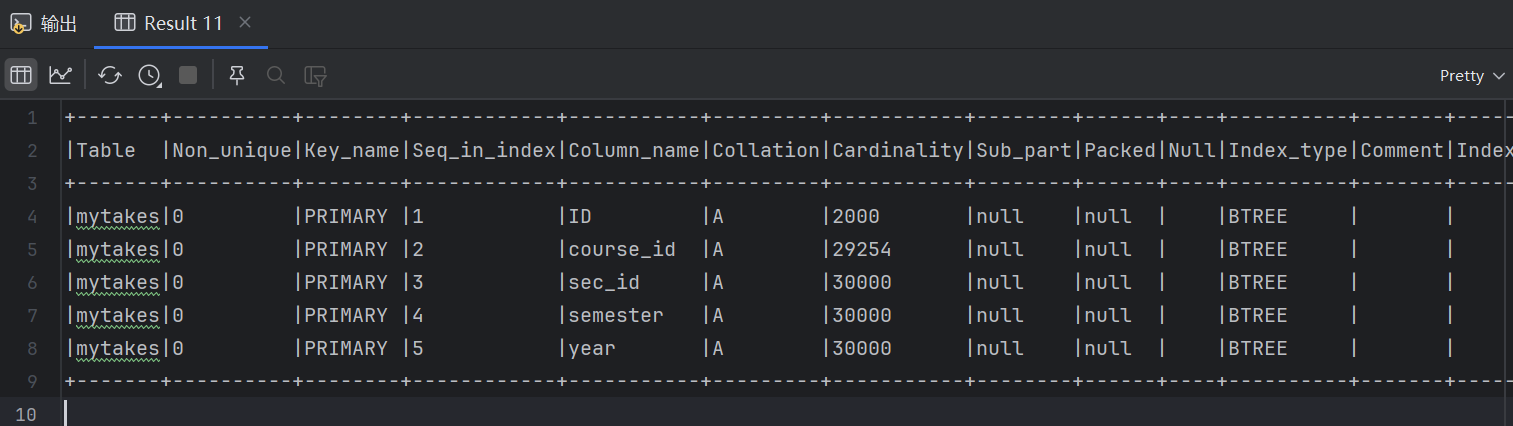
\includegraphics[width=13cm]{./images/3.检查mytakes的index.png}
		\caption{检查mytakes的index}
	\end{figure}
	
	与预期一致,可以继续下一步实验

	\begin{lstlisting}[language=sql, title=索引对查询性能的影响, tabsize=4]
	EXPLAIN SELECT * FROM mytakes where course_id='158';
	\end{lstlisting}
	
	得到以下结果:
	
	\begin{verbatim}
	+--+-----------+-------+----------+----+-------------+----+-------+----+-----+--------+-----------+
	|id|select_type|table  |partitions|type|possible_keys|key |key_len|ref |rows |filtered|Extra      |
	+--+-----------+-------+----------+----+-------------+----+-------+----+-----+--------+-----------+
	|1 |SIMPLE     |mytakes|null      |ALL |null         |null|null   |null|30000|10      |Using where|
	+--+-----------+-------+----------+----+-------------+----+-------+----+-----+--------+-----------+
	\end{verbatim}
	
	通过这个执行计划,我们可以看到在查询操作中,尽管使用了 WHERE 子句来限制结果,但MySQL 仍然对 mytakes 表进行了全表扫描,估计需要扫描30000行。这可能会影响查询性能,特别是在数据量较大的情况下。为了提高性能,可以考虑在 mytakes 表的 course\_id 列上创建适当的索引。

	\begin{lstlisting}[language=sql, title=索引对查询性能的影响, tabsize=4]
	EXPLAIN ANALYZE SELECT * FROM mytakes where course_id='158';
	\end{lstlisting}
	
	得到以下结果:
	
	\begin{verbatim}
	+----------------------------------------------------------------------------------------------+
	|EXPLAIN                                                                                       |
	+----------------------------------------------------------------------------------------------+
	|-> Filter: (mytakes.course_id = '158')  (cost=3024 rows=3000) 
	      (actual time=0.318..10.1 rows=577 loops=1)                                               |
	|-> Table scan on mytakes  (cost=3024 rows=30000) (actual time=0.305..8.84 rows=30000 loops=1) |
	+----------------------------------------------------------------------------------------------+
	\end{verbatim}
	
	通过这个执行计划,我们可以看到在查询操作中,尽管使用了 WHERE 子句来限制结果,但MySQL 仍然对 mytakes 表进行了全表扫描,扫描了30000行数据。实际执行时间从0.305秒到8.84秒不等,返回577行数据。这可能会影响查询性能,特别是在数据量较大的情况下。

	\begin{lstlisting}[language=sql, title=索引对查询性能的影响, tabsize=4]
	CREATE INDEX course_id ON mytakes(course_id);
	EXPLAIN SELECT * FROM mytakes where course_id='158';
	\end{lstlisting}
	
	得到以下结果:
	
	\begin{verbatim}
	+--+-----------+-------+----------+----+-------------+---------+-------+-----+----+--------+-----+
	|id|select_type|table  |partitions|type|possible_keys|key      |key_len|ref  |rows|filtered|Extra|
	+--+-----------+-------+----------+----+-------------+---------+-------+-----+----+--------+-----+
	|1 |SIMPLE     |mytakes|null      |ref |course_id    |course_id|34     |const|577 |100     |null |
	+--+-----------+-------+----------+----+-------------+---------+-------+-----+----+--------+-----+
	\end{verbatim}
	
	通过这个执行计划,我们可以看到在 mytakes 表的 course\_id 列上创建索引后,查询操作使用了该索引,显著减少了需要扫描的行数(从30000行减少到577行)。这表明查询性能得到了显著提高。
	
	\begin{lstlisting}[language=sql, title=索引对查询性能的影响, tabsize=4]
	EXPLAIN ANALYZE SELECT * FROM mytakes where course_id='158';
	\end{lstlisting}
	
	得到以下结果:
	
	\begin{verbatim}
	+------------------------------------------------------------------------------------+
	|EXPLAIN                                                                             |
	+------------------------------------------------------------------------------------+
	|-> Index lookup on mytakes using course_id (course_id='158')  (cost=130 rows=577)
	            (actual time=0.284..2.34 rows=577 loops=1)                               |
	+------------------------------------------------------------------------------------+
	\end{verbatim}
	
	通过这个执行计划,我们可以看到在 mytakes 表的 course\_id 列上创建索引后,查询操作使用了该索引,显著减少了需要扫描的行数(从30000行减少到577行)。这表明查询性能得到了显著提高。
	
	\begin{lstlisting}[language=sql, title=索引对查询性能的影响, tabsize=4]
	-- 分析索引失效原因
	EXPLAIN SELECT * FROM mytakes where course_id=158;
	\end{lstlisting}
	
	得到以下结果:
	
	\begin{verbatim}
	+--+-----------+-------+----------+----+-------------+----+-------+----+-----+--------+-----------+
	|id|select_type|table  |partitions|type|possible_keys|key |key_len|ref |rows |filtered|Extra      |
	+--+-----------+-------+----------+----+-------------+----+-------+----+-----+--------+-----------+
	|1 |SIMPLE     |mytakes|null      |ALL |course_id    |null|null   |null|30000|10      |Using where|
	+--+-----------+-------+----------+----+-------------+----+-------+----+-----+--------+-----------+
	\end{verbatim}
	
	在分析索引失效的原因时,我们发现尽管在 mytakes 表的 course\_id 列上创建了索引,但查询仍然进行了全表扫描。
	
	这可能是由于查询条件中的数据类型与索引列的数据类型不一致(例如,查询中使用了整数而索引列是字符串类型);
	
	或者查询没有使用索引的最左边的列(如果是复合索引);
	
	如果索引的选择性不高(即列中重复值很多),MySQL 可能认为全表扫描更有效。
	
	\begin{lstlisting}[language=sql, title=索引对查询性能的影响, tabsize=4]
	EXPLAIN ANALYZE SELECT * FROM mytakes where course_id=158;
	
	-- 删除索引
	DROP INDEX course_id ON mytakes;
	\end{lstlisting}
	
	得到以下结果:
	
	\begin{verbatim}
	+-------------------------------------------------------------------------------------+
	|EXPLAIN                                                                              |
	+-------------------------------------------------------------------------------------+
	|-> Filter: (mytakes.course_id = 158)  (cost=3024 rows=3000) 
	         (actual time=0.329..8.75 rows=577 loops=1)                                   |
	|-> Table scan on mytakes  (cost=3024 rows=30000) 
	         (actual time=0.31..7.49 rows=30000 loops=1)                                  |
	+-------------------------------------------------------------------------------------+
	\end{verbatim}
	
	尽管在mytakes表的course\_id列上创建了索引,但查询仍然进行了全表扫描,这可能是由于索引选择性不高、统计信息不准确或查询优化器的决策导致的。
	
	为了解决索引失效的问题,可以通过确保数据类型一致性、更新表统计信息、整理索引碎片或强制使用索引等方法来提高索引的使用效率,从而优化查询性能。
	
	\subsection{观察SELECT with INDEX -- ADVANCED查询性能}
	
	执行下列语句,观察索引对查询性能的影响,记录每条语句返回的结果并解释其完成的操作
	
	\begin{lstlisting}[language=sql, title=索引对查询性能的影响 - 总, tabsize=4]
	USE mydb;
	
	SHOW INDEXES FROM mysection; -- 执行结果要同上图所示,如有多余的index,请先drop删除掉
	EXPLAIN SELECT * FROM mysection where year=2006;
	EXPLAIN ANALYZE SELECT * FROM mysection where year=2006;
	EXPLAIN SELECT * FROM mysection where year=2006 and semester='Fall';
	EXPLAIN ANALYZE SELECT * FROM mysection where year=2006 and semester='Fall';
	EXPLAIN SELECT * FROM mysection where semester='Fall';
	EXPLAIN ANALYZE SELECT * FROM mysection where semester='Fall';
	
	CREATE INDEX composite_index on mysection(year,semester,building);
	EXPLAIN SELECT * FROM mysection where year=2006;
	EXPLAIN ANALYZE SELECT * FROM mysection where year=2006;
	EXPLAIN SELECT * FROM mysection where year=2006 and semester='Fall';
	EXPLAIN ANALYZE SELECT * FROM mysection where year=2006 and semester='Fall';
	
	-- 请分析不能使用上面建立的composite_index的原因
	EXPLAIN SELECT * FROM mysection where semester='Fall';
	EXPLAIN ANALYZE SELECT * FROM mysection where semester='Fall';	
	\end{lstlisting}
	
	接下来逐行执行,查看每行的结果并分析:
	
	\begin{lstlisting}[language=sql, title=索引对查询性能的影响, tabsize=4]
	SHOW INDEXES FROM mysection; -- 执行结果要同上图所示,如有多余的index,请先drop删除掉
	\end{lstlisting}
	
	得到结果如下图所示:
	
	\begin{figure}[H]
		\centering
		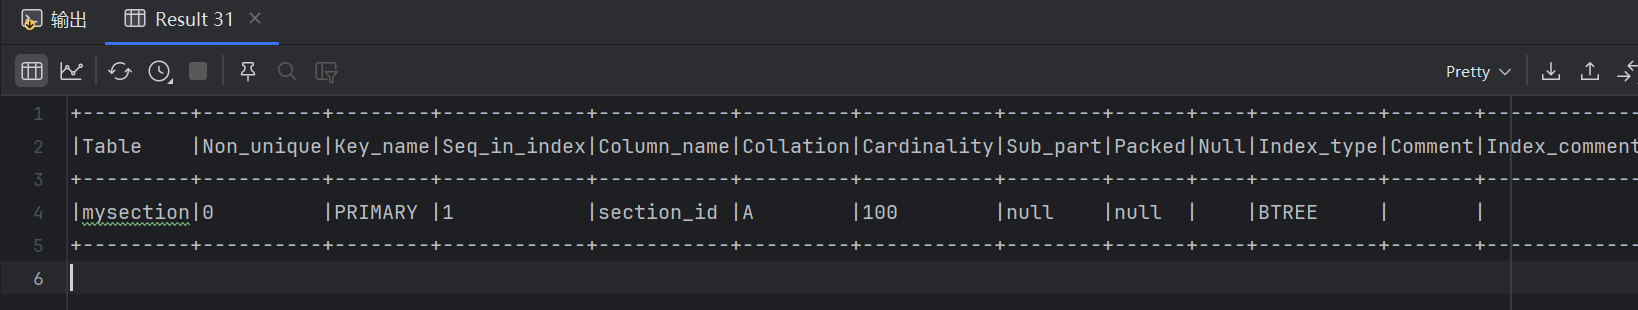
\includegraphics[width=13cm]{./images/4.检查mysection的index.png}
		\caption{检查mysection的index}
	\end{figure}
	
	与预期一致,可以继续下一步实验
	
	\begin{lstlisting}[language=sql, title=索引对查询性能的影响, tabsize=4]
	EXPLAIN SELECT * FROM mysection where year=2006;
	\end{lstlisting}
	
	得到以下结果:
	
	\begin{verbatim}
	+--+-----------+---------+----------+----+-------------+----+-------+----+----+--------+-----------+
	|id|select_type|table    |partitions|type|possible_keys|key |key_len|ref |rows|filtered|Extra      |
	+--+-----------+---------+----------+----+-------------+----+-------+----+----+--------+-----------+
	|1 |SIMPLE     |mysection|null      |ALL |null         |null|null   |null|100 |10      |Using where|
	+--+-----------+---------+----------+----+-------------+----+-------+----+----+--------+-----------+
	\end{verbatim}
	
	通过这个执行计划,我们可以看到在查询操作中,MySQL对mysection表进行了全表扫描,估计需要扫描100行。这表明查询性能可能受到影响,特别是在数据量较大的情况下。为了提高性能,可以考虑在mysection表的year列上创建适当的索引。
	
	\begin{lstlisting}[language=sql, title=索引对查询性能的影响, tabsize=4]
	EXPLAIN ANALYZE SELECT * FROM mysection where year=2006;
	\end{lstlisting}
	
	得到以下结果:
	
	\begin{verbatim}
	+--------------------------------------------------------------------------------------+
	|EXPLAIN                                                                                                                                                                                                   |
	+--------------------------------------------------------------------------------------+
	|-> Filter: (mysection.`year` = 2006)  (cost=10.2 rows=10) 
	            (actual time=0.0754..0.178 rows=13 loops=1)                                |
	|-> Table scan on mysection  (cost=10.2 rows=100) 
	             (actual time=0.0661..0.165 rows=100 loops=1)                              |
	+--------------------------------------------------------------------------------------+
	\end{verbatim}
	
	通过这个执行计划,我们可以看到在查询操作中,尽管使用了WHERE子句来限制结果,但MySQL仍然对mysection表进行了全表扫描,扫描了100行数据。实际执行时间较短,返回了13行数据。这表明查询性能可能受到影响,特别是在数据量较大的情况下。为了提高性能,可以考虑在mysection表的year列上创建适当的索引。
	
	\begin{lstlisting}[language=sql, title=索引对查询性能的影响, tabsize=4]
	EXPLAIN SELECT * FROM mysection where year=2006 and semester='Fall';
	\end{lstlisting}
	
	得到以下结果:
	
	\begin{verbatim}
	+--+-----------+---------+----------+----+-------------+----+-------+----+----+--------+-----------+
	|id|select_type|table    |partitions|type|possible_keys|key |key_len|ref |rows|filtered|Extra      |
	+--+-----------+---------+----------+----+-------------+----+-------+----+----+--------+-----------+
	|1 |SIMPLE     |mysection|null      |ALL |null         |null|null   |null|100 |1       |Using where|
	+--+-----------+---------+----------+----+-------------+----+-------+----+----+--------+-----------+
	\end{verbatim}
	
	通过这个执行计划,我们可以看到在查询操作中,MySQL对mysection表进行了全表扫描,估计需要扫描100行。这表明查询性能可能受到影响,特别是在数据量较大的情况下。为了提高性能,可以考虑在mysection表的year和semester列上创建适当的索引。
	
	\begin{lstlisting}[language=sql, title=索引对查询性能的影响, tabsize=4]
	EXPLAIN ANALYZE SELECT * FROM mysection where year=2006 and semester='Fall';
	\end{lstlisting}
	
	得到以下结果:
	
	\begin{verbatim}
	+--------------------------------------------------------------------------------------------+
	|EXPLAIN                                                                                     |
	+--------------------------------------------------------------------------------------------+
	|-> Filter: ((mysection.semester = 'Fall') and (mysection.`year` = 2006)) (cost=10.2 rows=1) 
	             (actual time=0.0417..0.119 rows=8 loops=1)                                      |
	|-> Table scan on mysection  (cost=10.2 rows=100) 
				 (actual time=0.0334..0.101 rows=100 loops=1)                                             |
	+--------------------------------------------------------------------------------------------+
	\end{verbatim}
	
	通过这个执行计划,我们可以看到在查询操作中,尽管使用了WHERE子句来限制结果,但MySQL仍然对mysection表进行了全表扫描,扫描了100行数据。实际执行时间较短,返回了8行数据。这表明查询性能可能受到影响,特别是在数据量较大的情况下。为了提高性能,可以考虑在mysection表的year和semester列上创建适当的索引。
	
	\begin{lstlisting}[language=sql, title=索引对查询性能的影响, tabsize=4]
	EXPLAIN SELECT * FROM mysection where semester='Fall';
	\end{lstlisting}
	
	得到以下结果:
	
	\begin{verbatim}
	+--+-----------+---------+----------+----+-------------+----+-------+----+----+--------+-----------+
	|id|select_type|table    |partitions|type|possible_keys|key |key_len|ref |rows|filtered|Extra      |
	+--+-----------+---------+----------+----+-------------+----+-------+----+----+--------+-----------+
	|1 |SIMPLE     |mysection|null      |ALL |null         |null|null   |null|100 |10      |Using where|
	+--+-----------+---------+----------+----+-------------+----+-------+----+----+--------+-----------+
	\end{verbatim}
	
	通过这个执行计划,我们可以看到在查询操作中,MySQL对mysection表进行了全表扫描,估计需要扫描100行。这表明查询性能可能受到影响,特别是在数据量较大的情况下。为了提高性能,可以考虑在mysection表的semester列上创建适当的索引。
	
	\begin{lstlisting}[language=sql, title=索引对查询性能的影响, tabsize=4]
	EXPLAIN ANALYZE SELECT * FROM mysection where semester='Fall';
	\end{lstlisting}
	
	得到以下结果:
	
	\begin{verbatim}
	+------------------------------------------------------------------------------------+
	|EXPLAIN                                                                             |
	+------------------------------------------------------------------------------------+
	|-> Filter: (mysection.semester = 'Fall')  (cost=10.2 rows=10) 
	           (actual time=0.037..0.111 rows=51 loops=1)                                |
	|-> Table scan on mysection  (cost=10.2 rows=100) 
	           (actual time=0.031..0.0951 rows=100 loops=1)                              |
	+------------------------------------------------------------------------------------+
	\end{verbatim}
	
	通过这个执行计划,我们可以看到在查询操作中,尽管使用了WHERE子句来限制结果,但MySQL仍然对mysection表进行了全表扫描,扫描了100行数据。实际执行时间较短,返回了51行数据。这表明查询性能可能受到影响,特别是在数据量较大的情况下。为了提高性能,可以考虑在mysection表的semester列上创建适当的索引。
	
	\begin{lstlisting}[language=sql, title=索引对查询性能的影响, tabsize=4]
	CREATE INDEX composite_index on mysection(year,semester,building);
	EXPLAIN SELECT * FROM mysection where year=2006;
	\end{lstlisting}
	
	得到以下结果:
	
	\begin{verbatim}
	+--+-----------+---------+----------+----+---------------+---------------+-------+-----+----+--------+-----+
	|id|select_type|table    |partitions|type|possible_keys  |key            |key_len|ref  |rows|filtered|Extra|
	+--+-----------+---------+----------+----+---------------+---------------+-------+-----+----+--------+-----+
	|1 |SIMPLE     |mysection|null      |ref |composite_index|composite_index|4      |const|13  |100     |null |
	+--+-----------+---------+----------+----+---------------+---------------+-------+-----+----+--------+-----+
	\end{verbatim}
	
	通过这个执行计划,我们可以看到在mysection表上创建复合索引后,查询使用了该索引,显著减少了需要扫描的行数(从100行减少到13行)。这表明查询性能得到了显著提高。
	
	\begin{lstlisting}[language=sql, title=索引对查询性能的影响, tabsize=4]
	EXPLAIN ANALYZE SELECT * FROM mysection where year=2006;
	\end{lstlisting}
	
	得到以下结果:
	
	\begin{verbatim}
	+------------------------------------------------------------------------------------+
	|EXPLAIN                                                                             |
	+------------------------------------------------------------------------------------+
	|-> Index lookup on mysection using composite_index (year=2006)  (cost=2.05 rows=13) 
	             (actual time=0.0585..0.0634 rows=13 loops=1)                            |
	+------------------------------------------------------------------------------------+
	\end{verbatim}
	
	通过这个执行计划,我们可以看到在mysection表上创建复合索引后,查询使用了该索引,显著减少了需要扫描的行数(从100行减少到13行)。这表明查询性能得到了显著提高,因为索引使得MySQL能够更快地定位到符合条件的行,从而减少了查询时间。
	
	\begin{lstlisting}[language=sql, title=索引对查询性能的影响, tabsize=4]
	EXPLAIN SELECT * FROM mysection where year=2006 and semester='Fall';
	\end{lstlisting}
	
	得到以下结果:
	
	\begin{verbatim}
	+--+-----------+---------+----------+----+---------------+---------------+-------+-----------+----+--------+-----+
	|id|select_type|table    |partitions|type|possible_keys  |key            |key_len|ref        |rows|filtered|Extra|
	+--+-----------+---------+----------+----+---------------+---------------+-------+-----------+----+--------+-----+
	|1 |SIMPLE     |mysection|null      |ref |composite_index|composite_index|30     |const,const|8   |100     |null |
	+--+-----------+---------+----------+----+---------------+---------------+-------+-----------+----+--------+-----+
	\end{verbatim}
	
	通过这个执行计划,我们可以看到在mysection表上创建复合索引后,查询使用了该索引,显著减少了需要扫描的行数(从100行减少到8行)。这表明查询性能得到了显著提高,因为索引使得MySQL能够更快地定位到符合条件的行,从而减少了查询时间。
	
	\begin{lstlisting}[language=sql, title=索引对查询性能的影响, tabsize=4]
	EXPLAIN ANALYZE SELECT * FROM mysection where year=2006 and semester='Fall';
	\end{lstlisting}
	
	得到以下结果:
	
	\begin{verbatim}
		+------------------------------------------------------------------------------------+
		|EXPLAIN                                                                             |
		+------------------------------------------------------------------------------------+
		|-> Index lookup on mysection using composite_index (year=2006, semester='Fall') 
		              (cost=1.55 rows=8) (actual time=0.0352..0.0385 rows=8 loops=1)         |
		+------------------------------------------------------------------------------------+
	\end{verbatim}
	
	通过这个执行计划,我们可以看到在mysection表上创建复合索引后,查询使用了该索引,显著减少了需要扫描的行数(从100行减少到8行)。这表明查询性能得到了显著提高,因为索引使得MySQL能够更快地定位到符合条件的行,从而减少了查询时间。
	
	\begin{lstlisting}[language=sql, title=索引对查询性能的影响, tabsize=4]
	-- 请分析不能使用上面建立的composite_index的原因
	EXPLAIN SELECT * FROM mysection where semester='Fall';
	\end{lstlisting}
	
	得到以下结果:
	
	\begin{verbatim}
	+--+-----------+---------+----------+----+-------------+----+-------+----+----+--------+-----------+
	|id|select_type|table    |partitions|type|possible_keys|key |key_len|ref |rows|filtered|Extra      |
	+--+-----------+---------+----------+----+-------------+----+-------+----+----+--------+-----------+
	|1 |SIMPLE     |mysection|null      |ALL |null         |null|null   |null|100 |10      |Using where|
	+--+-----------+---------+----------+----+-------------+----+-------+----+----+--------+-----------+
	\end{verbatim}
	
	在分析了mysection表的查询执行计划后,发现尽管存在一个复合索引composite\_index,但查询SELECT * FROM mysection WHERE semester='Fall'并未使用该索引,而是进行了全表扫描。这可能是因为查询条件没有使用索引的最左边的列(year),导致MySQL优化器认为全表扫描比使用索引更有效。为了提高查询性能,可以通过确保查询条件包含索引的最左边的列,或者使用FORCE INDEX强制使用索引,从而减少扫描的行数并提高查询效率。	
	\begin{lstlisting}[language=sql, title=索引对查询性能的影响, tabsize=4]
		EXPLAIN ANALYZE SELECT * FROM mysection where year=2006 and semester='Fall';
	\end{lstlisting}
	
	得到以下结果:
	
	\begin{verbatim}
	+-------------------------------------------------------------------------------------+
	|EXPLAIN                                                                              |
	+-------------------------------------------------------------------------------------+
	|-> Filter: (mysection.semester = 'Fall')  (cost=10.2 rows=10)
	            (actual time=0.0319..0.105 rows=51 loops=1)                               |
	|-> Table scan on mysection  (cost=10.2 rows=100) 
	            (actual time=0.03..0.0886 rows=100 loops=1)                               |
	+-------------------------------------------------------------------------------------+
	\end{verbatim}
	
	尽管在mysection表上创建了复合索引composite\_index,但查询SELECT * FROM mysection WHERE year=2006 AND semester='Fall'仍然进行了全表扫描,这是因为MySQL查询优化器决定不使用该索引。这可能是因为semester列的选择性较高(即该列中'Fall'值的行数相对较少),使得优化器认为全表扫描比使用索引更高效。此外,查询优化器可能基于统计信息和成本估算做出此决策,认为全表扫描在这种情况下更快。为了确保索引被使用,可以考虑更新表的统计信息,或者在查询中包含索引的最左边的列(year),以提高索引的使用率和查询性能。
	
	\subsection{观察SORT with INDEX查询性能}
	
	执行下列语句,观察索引对排序性能的影响,记录每条语句返回的结果并解释其完成的操作
	
	\begin{lstlisting}[language=sql, title=索引对排序性能的影响, tabsize=4]
	USE mydb;
	SHOW INDEXES FROM mytakes; -- 执行结果要同上图所示,如有多余的index,请先drop删除掉
	EXPLAIN SELECT * FROM mytakes ORDER BY course_id DESC LIMIT 10;
	EXPLAIN ANALYZE SELECT * FROM mytakes ORDER BY course_id DESC LIMIT 10;
	CREATE INDEX course_id ON mytakes(course_id);
	EXPLAIN SELECT * FROM mytakes ORDER BY course_id DESC LIMIT 10;
	EXPLAIN ANALYZE SELECT * FROM mytakes ORDER BY course_id DESC LIMIT 10;	
	\end{lstlisting}
	
	接下来逐行执行,查看每行的结果并分析:
	
	\begin{lstlisting}[language=sql, title=索引对查询性能的影响, tabsize=4]
	SHOW INDEXES FROM mytakes; -- 执行结果要同上图所示,如有多余的index,请先drop删除掉
	\end{lstlisting}
	
	得到结果如下图所示:
	
	\begin{figure}[H]
		\centering
		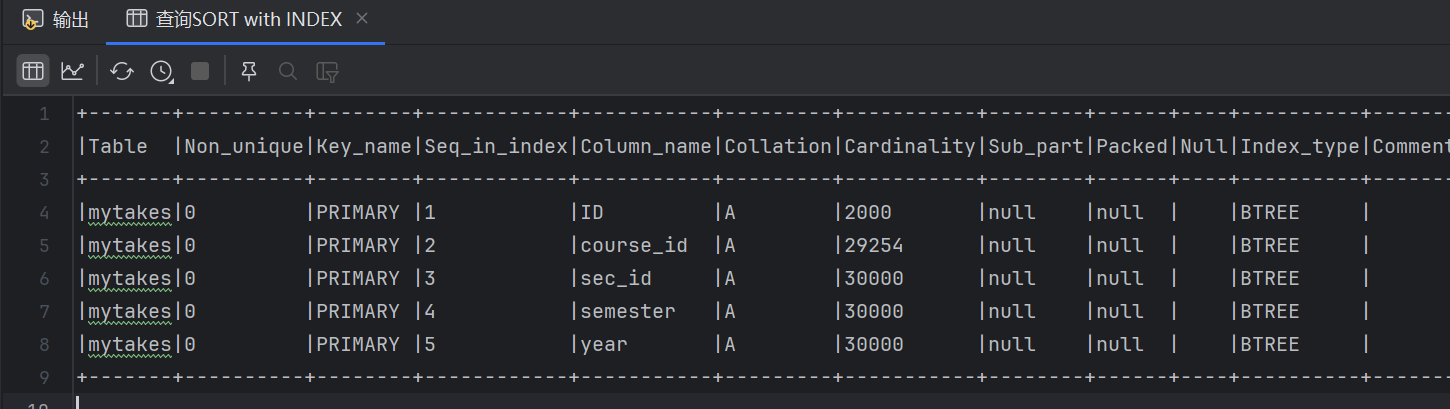
\includegraphics[width=13cm]{./images/5.检查mytakes的index.png}
		\caption{检查mytakes的index}
	\end{figure}
	
	与预期一致,可以继续下一步实验
	
	\begin{lstlisting}[language=sql, title=索引对查询性能的影响, tabsize=4]
	EXPLAIN SELECT * FROM mytakes ORDER BY course_id DESC LIMIT 10;
	\end{lstlisting}
	
	得到以下结果:
	
	\begin{verbatim}
	+--+-----------+-------+----------+----+-------------+----+-------+----+-----+--------+--------------+
	|id|select_type|table  |partitions|type|possible_keys|key |key_len|ref |rows |filtered|Extra         |
	+--+-----------+-------+----------+----+-------------+----+-------+----+-----+--------+--------------+
	|1 |SIMPLE     |mytakes|null      |ALL |null         |null|null   |null|30000|100     |Using filesort|
	+--+-----------+-------+----------+----+-------------+----+-------+----+-----+--------+--------------+
	\end{verbatim}
	
	该查询从mytakes表中选择所有列,并按course\_id列的值降序排序,限制返回前10行。EXPLAIN关键字用于获取查询的执行计划,结果显示查询进行了全表扫描(type为ALL),没有使用任何索引,预计读取30000行数据,并使用文件排序(Using filesort)来完成排序操作。
	
	这表明查询性能可能受到影响,特别是在数据量较大的情况下。为了提高性能,可以考虑在course\_id列上创建索引,以减少扫描的行数并提高排序效率。
	
	\begin{lstlisting}[language=sql, title=索引对查询性能的影响, tabsize=4]
	EXPLAIN ANALYZE SELECT * FROM mytakes ORDER BY course_id DESC LIMIT 10;
	\end{lstlisting}
	
	得到以下结果:
	
	\begin{verbatim}
	+--------------------------------------------------------------------------------------------+
	|EXPLAIN                                                                                     |
	+--------------------------------------------------------------------------------------------+
	|-> Limit: 10 row(s)  (cost=3024 rows=10) (actual time=13.9..13.9 rows=10 loops=1)           |
	|-> Sort: mytakes.course_id DESC, limit input to 10 row(s) per chunk  (cost=3024 rows=30000) 
	            (actual time=13.9..13.9 rows=10 loops=1)                                         |
	|-> Table scan on mytakes  (cost=3024 rows=30000) 
	            (actual time=0.337..9.02 rows=30000 loops=1)                                     |
	+--------------------------------------------------------------------------------------------+
	\end{verbatim}
	
	这段代码展示了一个SQL查询的执行计划,该查询从mytakes表中选择所有列,按course\_id列的值降序排序,并限制返回前10行。EXPLAIN ANALYZE关键字用于获取查询的执行计划和实际执行的详细信息,结果显示查询进行了全表扫描,没有使用任何索引,预计读取30000行数据,并且需要进行排序操作。
	
	实际执行时间显示了各个步骤的耗时,包括应用LIMIT条件、排序以及全表扫描的时间。这表明查询性能可能受到影响,特别是在数据量较大的情况下。为了提高性能,可以考虑在course\_id列上创建索引,以减少扫描的行数并提高排序效率。
	
	\begin{lstlisting}[language=sql, title=索引对查询性能的影响, tabsize=4]
	EXPLAIN SELECT * FROM mytakes ORDER BY course_id DESC LIMIT 10;
	\end{lstlisting}
	
	得到以下结果:
	
	\begin{verbatim}
	+--+-----------+-------+----------+-----+-------------+---------+-------+----+----+--------+-------------------+
	|id|select_type|table  |partitions|type |possible_keys|key      |key_len|ref |rows|filtered|Extra              |
	+--+-----------+-------+----------+-----+-------------+---------+-------+----+----+--------+-------------------+
	|1 |SIMPLE     |mytakes|null      |index|null         |course_id|34     |null|10  |100     |Backward index scan|
	+--+-----------+-------+----------+-----+-------------+---------+-------+----+----+--------+-------------------+
	\end{verbatim}
	
	这段代码展示了在mytakes表上创建了course\_id索引后,执行一个按course\_id降序排序并限制返回前10行的查询,并使用EXPLAIN来分析查询的执行计划。结果显示查询使用了course\_id索引来优化排序操作,显著减少了需要扫描的行数,从而提高了查询性能。
	
	\begin{lstlisting}[language=sql, title=索引对查询性能的影响, tabsize=4]
	EXPLAIN ANALYZE SELECT * FROM mytakes ORDER BY course_id DESC LIMIT 10;
	\end{lstlisting}
	
	得到以下结果:
	
	\begin{verbatim}
	+----------------------------------------------------------------------------------------+
	|EXPLAIN                                                                                 |
	+----------------------------------------------------------------------------------------+
	|-> Limit: 10 row(s)  (cost=0.00842 rows=10) (actual time=0.21..0.213 rows=10 loops=1)   |
	|-> Index scan on mytakes using course_id (reverse)  (cost=0.00842 rows=10)
	             (actual time=0.209..0.212 rows=10 loops=1)                                  |
	+----------------------------------------------------------------------------------------+
	\end{verbatim}
	
	这段代码展示了在mytakes表上创建了course\_id索引后,执行一个按course\_id降序排序并限制返回前10行的查询,并使用EXPLAIN ANALYZE来分析查询的执行计划。结果显示查询有效地使用了course\_id索引进行排序和限制返回结果,显著减少了查询成本和执行时间,表明索引在优化查询性能方面发挥了重要作用。
	
	\subsection{索引性能测试 - 导入数据库}
	
	首先来看一下要求与我设想的解决方案:
	
	\begin{tcolorbox}[title = {要求与方案}, colback = blue!25!white, colframe = blue!75!black]
		\begin{enumerate}
			\item 索引类型:无索引、唯一索引(\texttt{btree}、\texttt{hash})、非唯一索引(\texttt{btree}、\texttt{hash}) -> 通过不采用索引,给id加索引,给age加索引来完成
			\item 查询类型:等值查询、范围查询 -> 通过查询唯一id或非唯一的年龄范围
			\item 查询结果集:单条、少量(<10)、大量(1,000) -> 根据实际的数据集数量来筛选LIMIT的数量
			\item 数据集规模:100、10,000、1,000,000 -> 使用不同大小的数据集来解决
		\end{enumerate}
	\end{tcolorbox}
	
	这里我使用的数据库是从kaggle上下载下来的lung-cancer-dataset(dataset\_med),
	
	参考地址:\textbf{https://www.kaggle.com/datasets/amankumar094/lung-cancer-dataset}
	
	\begin{figure}[H]
		\centering
		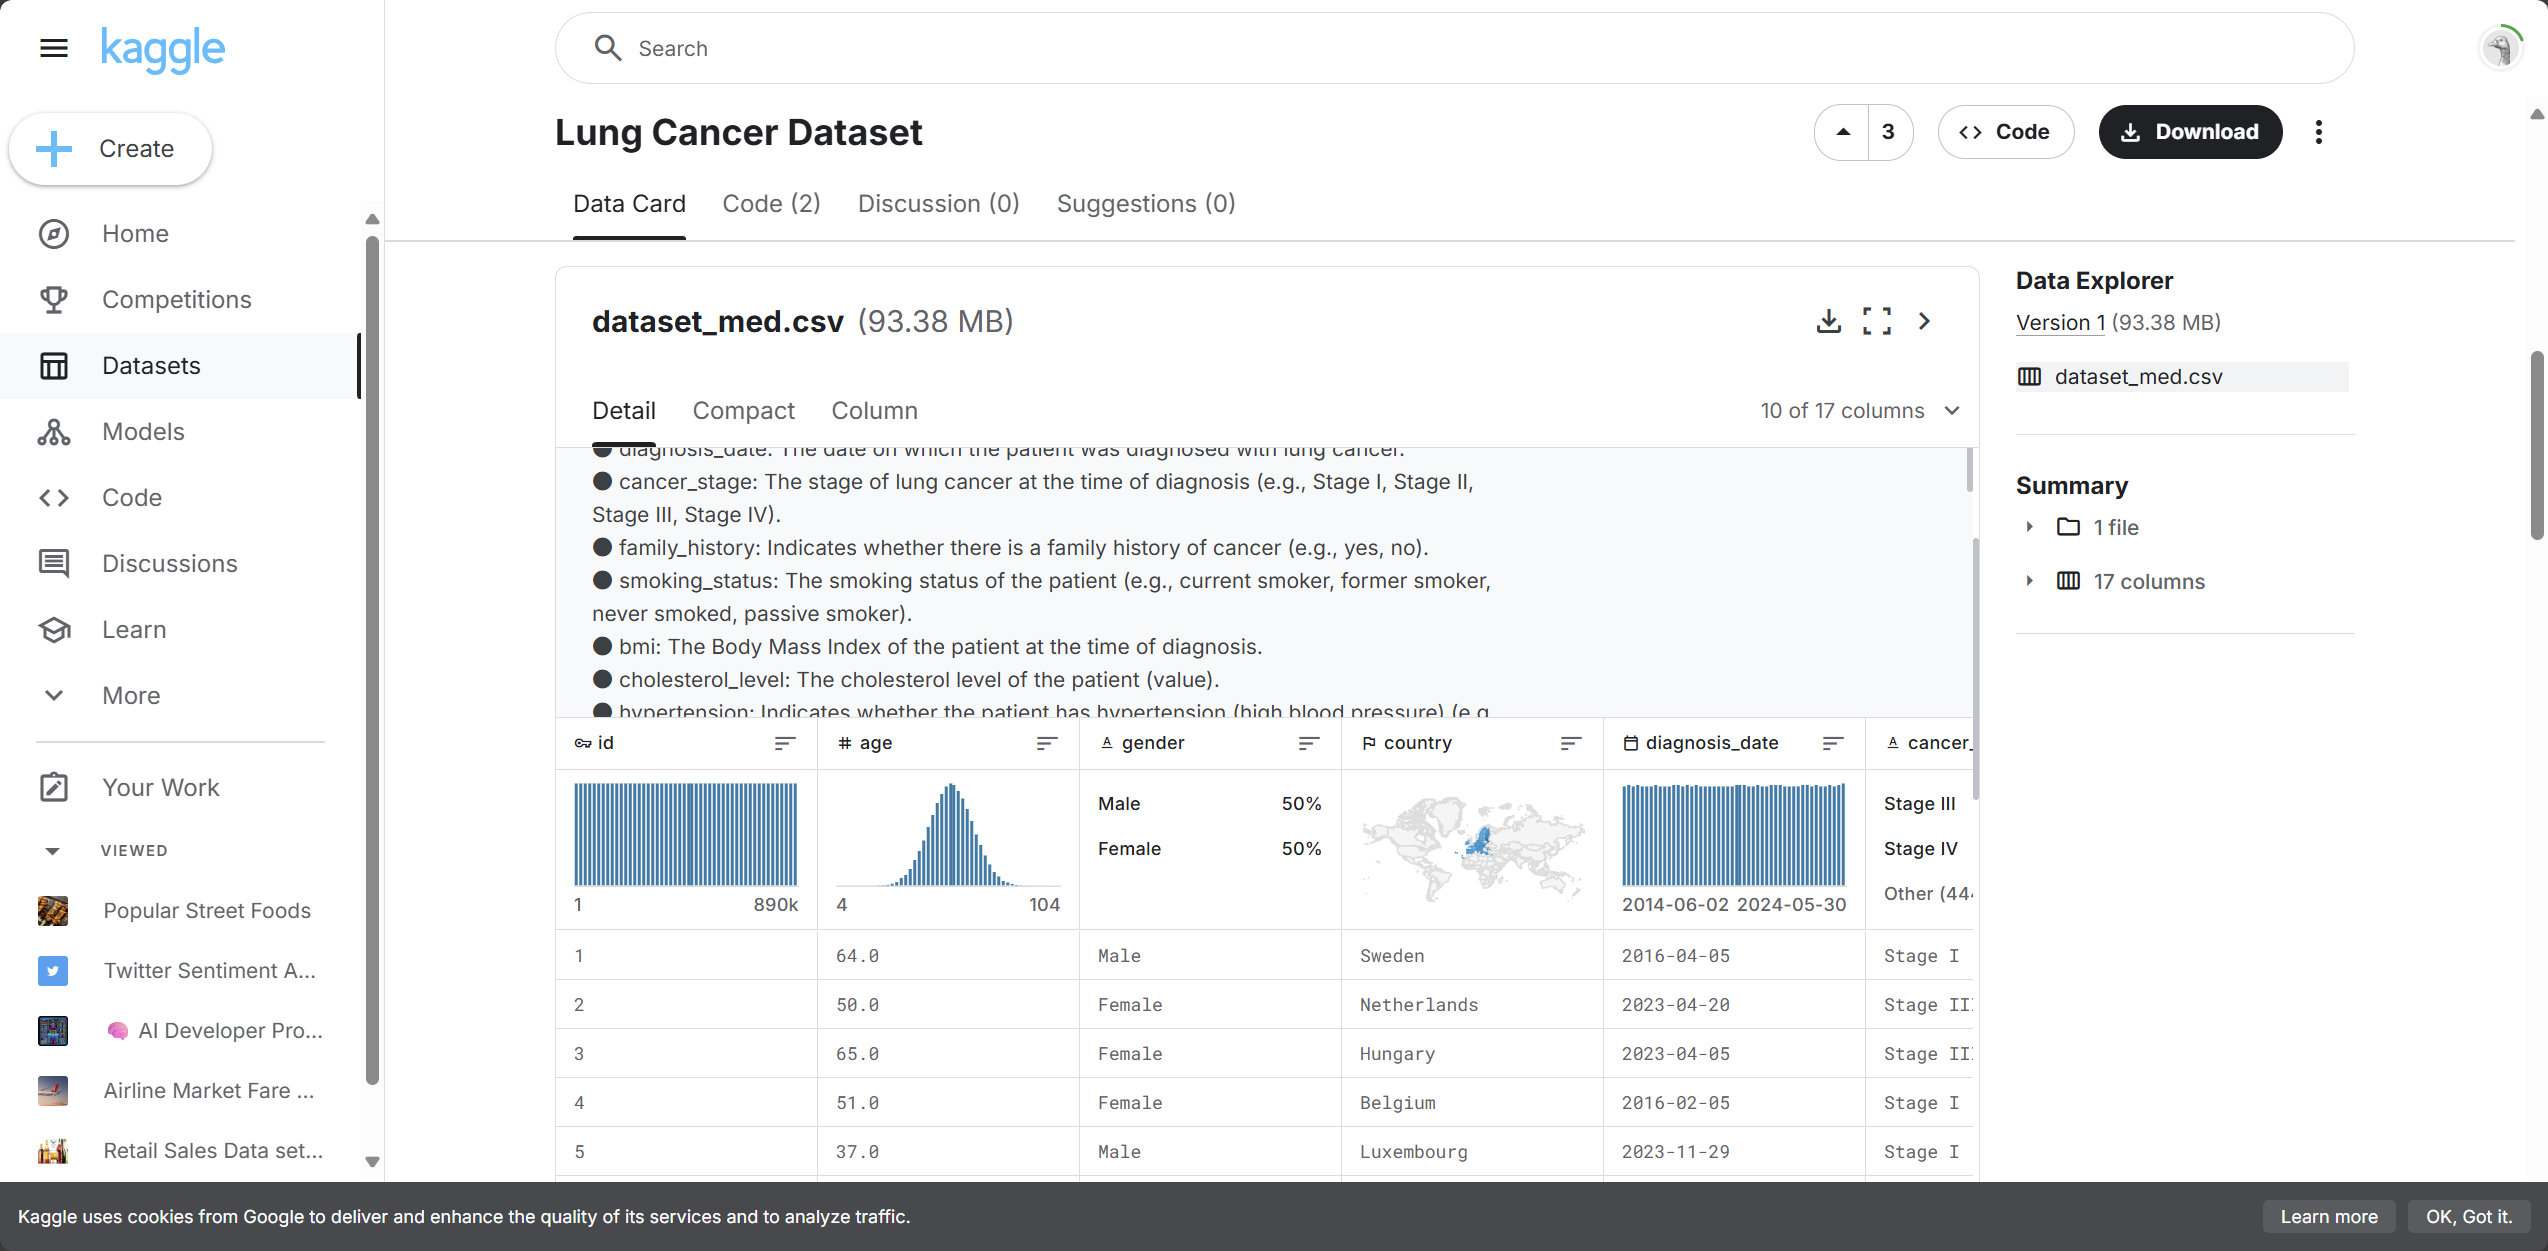
\includegraphics[width=15cm]{./images/6.kaggle官网上找到的合适数据集.png}
		\caption{kaggle官网上找到的合适数据集}
	\end{figure}
	
	下载的csv如图所示,数据总共约890,000个元组数据,此处只展示部分
	
	\begin{figure}[H]
		\centering
		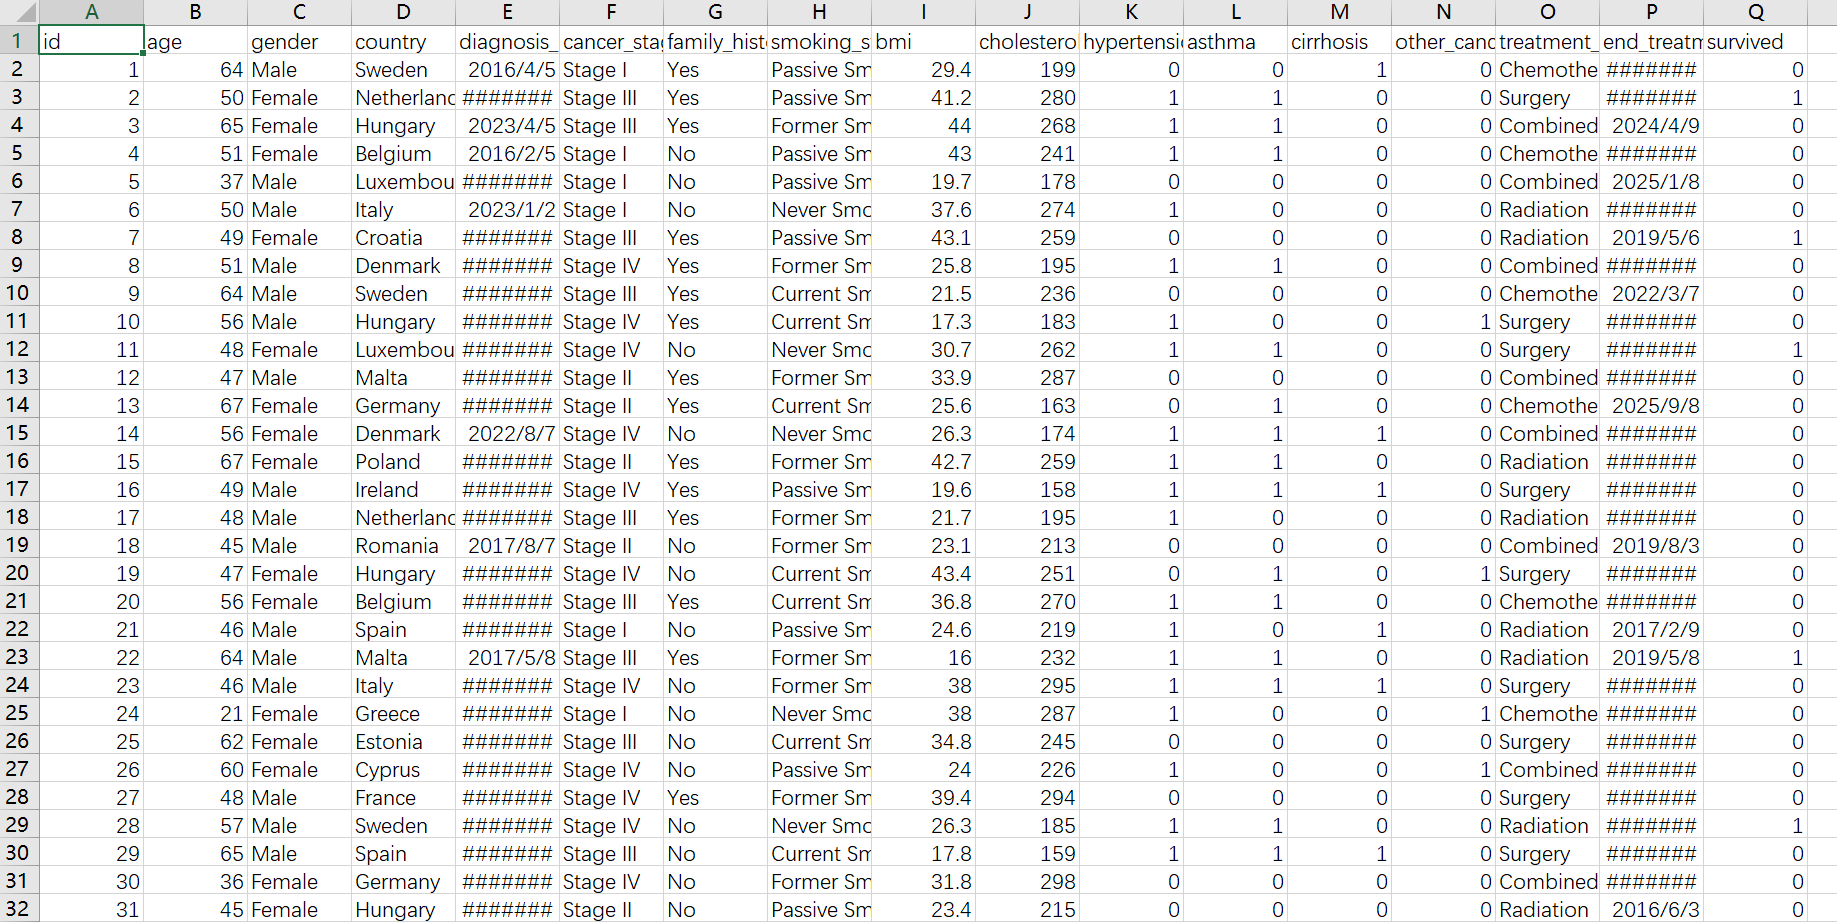
\includegraphics[width=15cm]{./images/7.dataset_med.png}
		\caption{dataset\_med.csv}
	\end{figure}
	
	使用sql语句将csv文件导入需要的数据库
	
	首先创建数据集对应的表格,代码如下所示:
	
	\begin{lstlisting}[language=sql, title=使用sql语句将csv文件导入需要的数据库, tabsize=4]
	create table `lab-5_dataset_med`.dataset_med
	(
		id                 integer          null,
		age                double precision null,
		gender             text             null,
		country            text             null,
		diagnosis_date     text             null,
		cancer_stage       text             null,
		family_history     text             null,
		smoking_status     text             null,
		bmi                double precision null,
		cholesterol_level  integer          null,
		hypertension       integer          null,
		asthma             integer          null,
		cirrhosis          integer          null,
		other_cancer       integer          null,
		treatment_type     text             null,
		end_treatment_date text             null,
		survived           text             null
	);
	\end{lstlisting}
	
	导入以后利用以下语句来检验是否导入成功:
	
	\begin{lstlisting}[language=sql, title=检验是否导入成功, tabsize=4]
	SELECT * FROM dataset_med LIMIT 10;
	\end{lstlisting}
	
	\begin{figure}[H]
		\centering
		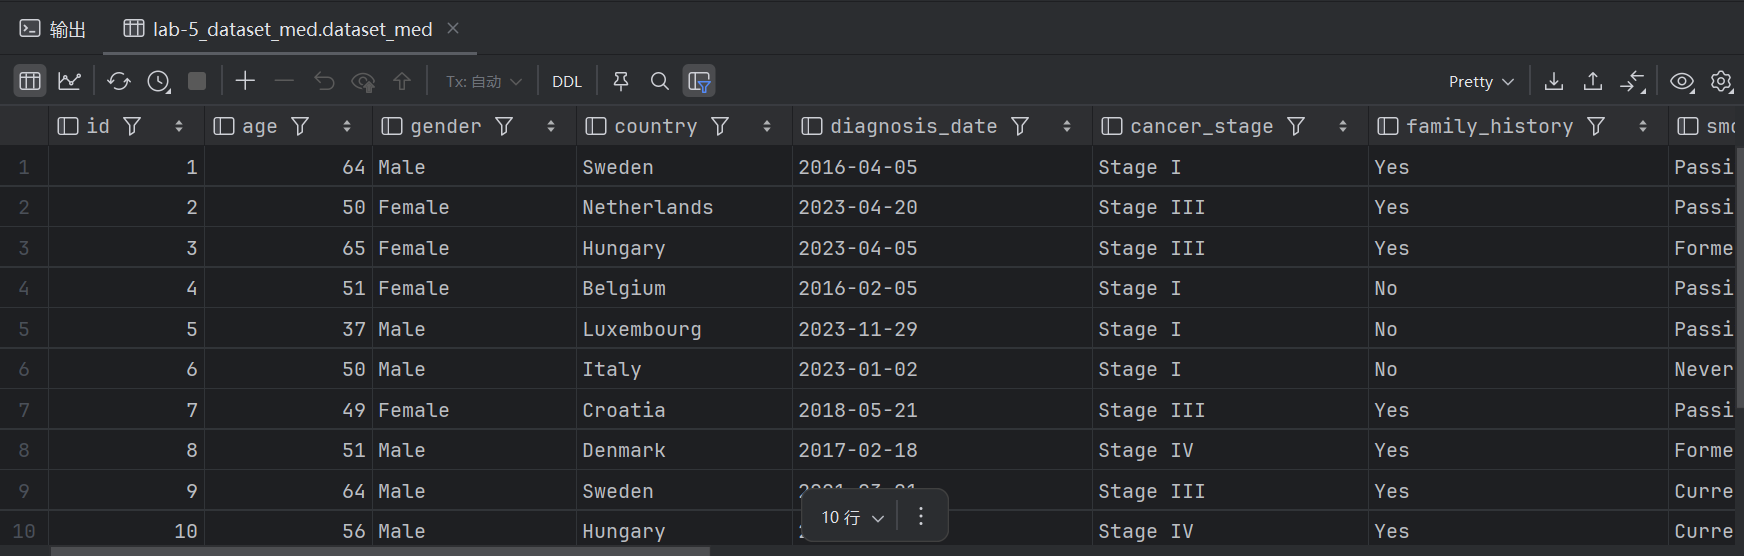
\includegraphics[width=13cm]{./images/8.检验导入结果.png}
		\caption{检验导入结果}
	\end{figure}
	
	这里的结果与csv表格内的内容相同,符合预期,可以继续实验
	
	由于需要三种数据规模的数据集,所以这里按照同样的方法导入三次。
	
	\subsection{索引性能测试 - 数据集重新整理}
	
	由于实验需要的数据集规模为:100、10,000、1,000,000,所以我需要将多余的部分删去,使用以下代码:
	
	\begin{lstlisting}[language=sql, title=删去多余的数据, tabsize=4]
	DELETE FROM dataset_med
	WHERE id > 100;
	
	DELETE FROM dataset_med_2
	WHERE id > 10000;
	\end{lstlisting}
	
	至此,数据已经全部准备完毕,可以开始测试索引性能了。
	
	\subsection{索引性能测试 - 测试}
	
	\subsubsection{等值查询,并包含无索引和唯一索引}
	
	以下是等值查询,并包含无索引和唯一索引内的完整代码,接下来会逐条展示结果并分析
	
	\begin{lstlisting}[language=sql, title=等值查询,并包含无索引和唯一索引, tabsize=4]
	-- 等值查询,包含无索引和唯一索引
	DROP INDEX id ON dataset_med;
	DROP INDEX age ON dataset_med;
	EXPLAIN ANALYZE SELECT * FROM dataset_med WHERE id = 10;  -- 无索引
	CREATE UNIQUE INDEX id ON dataset_med (id);  -- 在id列上创建唯一索引,因为id列中的每个值都是唯一的。
	EXPLAIN ANALYZE SELECT * FROM dataset_med ORDER BY id LIMIT 1;  -- 唯一索引
	\end{lstlisting}
	
	接下来逐条展示结果并分析
	
	\begin{lstlisting}[language=sql, title=无索引等值查询, tabsize=4]
	EXPLAIN ANALYZE SELECT * FROM dataset_med WHERE id = 10;  -- 无索引等值查询
	\end{lstlisting}
	
	展示结果为
	
	\begin{verbatim}
	+------------------------------------------------------------------------------------------------+
	|EXPLAIN                                                                                         |
	+--------------------------------------------------------------------------------------------------------------------------------------------------------------------------------------------------+
	|-> Filter: (dataset_med.id = 10)  (cost=3098 rows=1) (actual time=0.0455..0.165 rows=1 loops=1) |
	|-> Table scan on dataset_med  (cost=3098 rows=1) (actual time=0.0282..0.151 rows=100 loops=1)   |
	+------------------------------------------------------------------------------------------------+
	\end{verbatim}
	
	通过这个执行计划,我们可以看到在 dataset\_med 表上没有使用索引,而是进行了全表扫描。尽管如此,由于数据量较小(100行),查询性能影响不大。然而,如果表中的数据量更大,创建适当的索引可以显著提高查询性能。例如,可以在 id 列上创建索引来优化查询
	
	\begin{lstlisting}[language=sql, title=唯一索引等值查询, tabsize=4]
	CREATE UNIQUE INDEX id ON dataset_med (id);  -- 在id列上创建唯一索引,因为id列中的每个值都是唯一的。
	EXPLAIN ANALYZE SELECT * FROM dataset_med ORDER BY id LIMIT 1;  -- 唯一索引等值查询
	\end{lstlisting}
	
	展示结果为
	
	\begin{verbatim}
	+------------------------------------------------------------------------------------------------+
	|EXPLAIN                                                                                         |
	+------------------------------------------------------------------------------------------------+
	|-> Limit: 1 row(s)  (cost=3098 rows=1) (actual time=0.0373..0.0373 rows=1 loops=1)                |
	|-> Index scan on dataset_med using id  (cost=3098 rows=1) 
	            (actual time=0.0363..0.0363 rows=1 loops=1)                                          |
	+------------------------------------------------------------------------------------------------+
	\end{verbatim}
	
	通过这个执行计划,我们可以看到在dataset\_med表上创建唯一索引后,查询使用了该索引,显著减少了需要扫描的行数(从100行减少到1行)。这表明查询性能得到了显著提高,因为索引使得MySQL能够更快地定位到符合条件的行,从而减少了查询时间。创建唯一索引可以优化等值查询,特别是当查询条件涉及唯一列时。
	
	\subsubsection{范围查询,并包含无索引和非唯一索引}
	
	以下是范围查询,包含无索引和非唯一索引的完整代码,接下来会逐条展示结果并分析
	
	\begin{lstlisting}[language=sql, title=范围查询,包含无索引和非唯一索引, tabsize=4]
	-- 范围查询,包含无索引和非唯一索引
	DROP INDEX id ON dataset_med;
	DROP INDEX age ON dataset_med;
	EXPLAIN ANALYZE SELECT * FROM dataset_med WHERE age = 10;  -- 无索引
	CREATE INDEX age ON dataset_med (age);  -- 在age列上创建非唯一索引,因为age列中可能存在重复值。
	EXPLAIN ANALYZE SELECT * FROM dataset_med ORDER BY age LIMIT 10;  -- 非唯一索引
	\end{lstlisting}
	
	接下来逐条展示结果并分析
	
	\begin{lstlisting}[language=sql, title=无索引范围查询, tabsize=4]
	EXPLAIN SELECT * FROM dataset_med WHERE age = 10;  -- 无索引
	\end{lstlisting}
	
	展示结果为
	
	\begin{verbatim}
	+------------------------------------------------------------------------------------------------+
	|EXPLAIN                                                                                         |
	+------------------------------------------------------------------------------------------------+
	|-> Filter: (dataset_med.age = 10)  (cost=3098 rows=1) (actual time=0.315..0.315 rows=0 loops=1) |
	|-> Table scan on dataset_med  (cost=3098 rows=1) (actual time=0.0462..0.286 rows=100 loops=1)   |
	+------------------------------------------------------------------------------------------------+
	\end{verbatim}
	
	通过这个执行计划,我们可以看到在dataset\_med表上没有使用索引,而是进行了全表扫描。尽管如此,由于数据量较小(100行),查询性能影响不大。然而,如果表中的数据量更大,创建适当的索引可以显著提高查询性能。例如,可以在age列上创建索引来优化查询
	
	\begin{lstlisting}[language=sql, title=非唯一索引范围查询, tabsize=4]
	CREATE INDEX age ON dataset_med (age);  -- 在age列上创建非唯一索引,因为age列中可能存在重复值。
	EXPLAIN ANALYZE SELECT * FROM dataset_med ORDER BY age LIMIT 10;  -- 非唯一索引
	\end{lstlisting}
	
	展示结果为
	
	\begin{verbatim}
	+------------------------------------------------------------------------------------------------+
	|EXPLAIN                                                                                         |
	+------------------------------------------------------------------------------------------------+
	|-> Limit: 10 row(s)  (cost=3098 rows=1) (actual time=0.032..0.0541 rows=10 loops=1)             |
	|-> Index scan on dataset_med using age  (cost=3098 rows=1)
	            (actual time=0.0312..0.0528 rows=10 loops=1)                                         |
	+------------------------------------------------------------------------------------------------+
	\end{verbatim}
	
	通过这个执行计划,我们可以看到在dataset\_med表上创建非唯一索引后,查询使用了该索引,显著减少了需要扫描的行数(从100行减少到10行)。这表明查询性能得到了显著提高,因为索引使得MySQL能够更快地定位到符合条件的行,从而减少了查询时间。创建非唯一索引可以优化范围查询,特别是当查询条件涉及可能存在重复值的列时
	
	\subsubsection{不同数据集大小与查询结果大小}
	
	以下是不同数据集大小与查询结果大小的完整代码,接下来会逐条展示结果并分析
	
	\begin{lstlisting}[language=sql, title=不同数据集大小与查询结果大小, tabsize=4]
	-- 不同数据集大小与查询结果大小
	CREATE UNIQUE INDEX id ON dataset_med (id);  -- 在id列上创建唯一索引,因为id列中的每个值都是唯一的。
	EXPLAIN ANALYZE SELECT * FROM dataset_med ORDER BY id LIMIT 1;  -- 数据集规模100,查询单条结果
	EXPLAIN ANALYZE SELECT * FROM dataset_med_2 ORDER BY id LIMIT 10;  -- 数据集规模10,000,查询少量结果
	EXPLAIN ANALYZE SELECT * FROM dataset_med_3 ORDER BY id LIMIT 1000;  -- 数据集规模1,000,000,查询大量结果
	\end{lstlisting}
	
	接下来逐条展示结果并分析
	
	\begin{lstlisting}[language=sql, title=数据集规模100,查询单条结果, tabsize=4]
	EXPLAIN ANALYZE SELECT * FROM dataset_med ORDER BY id LIMIT 1;  -- 数据集规模100,查询单条结果
	\end{lstlisting}
	
	展示结果为
	
	\begin{verbatim}
	+------------------------------------------------------------------------------------------------+
	|EXPLAIN                                                                                         |
	+------------------------------------------------------------------------------------------------+
	|-> Limit: 1 row(s)  (cost=3098 rows=1) (actual time=0.0363..0.0364 rows=1 loops=1)              |
	|-> Index scan on dataset_med using id  (cost=3098 rows=1)
	           (actual time=0.0354..0.0354 rows=1 loops=1)                                           |
	+------------------------------------------------------------------------------------------------+
	\end{verbatim}
	
	通过这个执行计划,我们可以看到在dataset\_med表上创建了id列的索引后,查询使用了该索引,显著减少了需要扫描的行数(从100行减少到1行)。这表明查询性能得到了显著提高,因为索引使得MySQL能够更快地定位到符合条件的行,从而减少了查询时间。创建索引可以优化等值查询,特别是当查询条件涉及主键列时
	
	\begin{lstlisting}[language=sql, title=数据集规模10000,查询少量结果, tabsize=4]
	CREATE UNIQUE INDEX id ON dataset_med_2 (id);  -- 在id列上创建唯一索引,因为id列中的每个值都是唯一的。
	EXPLAIN ANALYZE SELECT * FROM dataset_med_2 ORDER BY id LIMIT 10;  -- 数据集规模10,000,查询少量结果
	\end{lstlisting}
	
	展示结果为
	
	\begin{verbatim}
	+---------------------------------------------------------------------------------------------+
	|EXPLAIN                                                                                      |
	+---------------------------------------------------------------------------------------------+          |
	|-> Limit: 10 row(s)  (cost=4957 rows=1) (actual time=1.46..1.51 rows=10 loops=1)                                          |
	|-> Index scan on dataset_med_2 using id  (cost=4957 rows=1)
	            (actual time=1.46..1.51 rows=10 loops=1)                                          |
	+---------------------------------------------------------------------------------------------+
	\end{verbatim}
	
	通过这个执行计划,我们可以看到在dataset\_med\_2表上创建唯一索引后,查询使用了该索引,显著减少了需要扫描的行数(从10000行减少到10行)。这表明查询性能得到了显著提高,因为索引使得MySQL能够更快地定位到符合条件的行,从而减少了查询时间。创建唯一索引可以优化等值查询,特别是当查询条件涉及主键列时。
	
	\begin{lstlisting}[language=sql, title=数据集规模1000000,查询大量结果, tabsize=4]
	CREATE UNIQUE INDEX id ON dataset_med_3 (id);  -- 在id列上创建唯一索引,因为id列中的每个值都是唯一的。
	EXPLAIN ANALYZE SELECT * FROM dataset_med_3 ORDER BY id LIMIT 1000;  -- 数据集规模1,000,000,查询大量结果
	\end{lstlisting}
	
	展示结果为
	
	\begin{verbatim}
	+-----------------------------------------------------------------------------------------+
	|EXPLAIN                                                                                  |
	+-----------------------------------------------------------------------------------------+
	|-> Limit: 1000 row(s)  (cost=9.67 rows=1000) (actual time=1.82..6.13 rows=1000 loops=1)                                    |
	|-> Index scan on dataset_med_3 using id  (cost=9.67 rows=1000)
	            (actual time=1.82..6.09 rows=1000 loops=1)                                    |
	+-----------------------------------------------------------------------------------------+
	\end{verbatim}
	
	通过这个执行计划,我们可以看到在dataset\_med\_3表上创建唯一索引后,查询使用了该索引,显著减少了需要扫描的行数(从100万行减少到1000行)。这表明查询性能得到了显著提高,因为索引使得MySQL能够更快地定位到符合条件的行,从而减少了查询时间。创建唯一索引可以优化等值查询,特别是当查询条件涉及主键列时
	
	\section{存在的问题及解决方案}
	
	\subsection{存在的问题:}
	
	\begin{enumerate}[noitemsep, label={{\arabic*})}]
		\item \textbf{数据获取困难}: 在寻找符合特定需求的数据集时,常常难以找到包含100、10000和1000000条记录的数据集。这些数据集的规模差异较大,导致获取过程复杂且耗时;
		\item \textbf{数据分配策略不明确}: 即使成功获取了数据集,如何根据具体需求进行合理分配仍然是一个挑战。需要制定科学合理的分配策略,以确保数据的有效利用;
		\item \textbf{SQL实验操作不熟悉}: 在数据集分配完成后,如何使用SQL语句进行实验操作成为一个难题。缺乏相关经验可能导致实验结果不准确或效率低下;
	\end{enumerate}\textbf{}
	
	\subsection{解决方案:}
	
	\begin{enumerate}[noitemsep, label={{\arabic*})}]
		\item \textbf{数据集分段处理}:考虑到需要验证每次实验结果的准确性和方便性,我决定使用同一个数据集进行分段处理,将其分为三个子数据集。通过这种方式,可以确保实验结果的一致性和可比性。我在Kaggle官网(https://www.kaggle.com/)上利用筛选条件找到了合适的数据集,例如dataset\_med;
		\item \textbf{数据集来源一致性}: 为了确保实验的可重复性,我下载了一个包含89万条记录的数据库,并在此基础上进行分割存储。通过删除不需要的部分,生成了包含100、10000和1000000条记录的三个数据集。这种方法不仅简化了数据管理,还提高了实验的灵活性;
		\item \textbf{代码学习和实验分析}: 由于第一部分的实验中老师提供了所有的代码,我针对这些代码进行了深入学习。这包括创建索引和使用索引进行查询的操作。此外,我还结合之前的实验阅读了EXPLAIN和EXPLAIN ANALYSE的结果,以理解每个结果所展示的含义。这不仅提高了我的SQL技能,还增强了对数据库性能优化的理解;
	\end{enumerate}\textbf{}
	
	\section{实验小结}
	
	\subsection{实验目的}
	本实验旨在评估和分析MySQL索引对查询性能的影响。通过在不同数据集规模和索引类型下,测试等值查询和范围查询的性能,以确定索引在提高查询效率中的作用。
	
	\subsection{实验方法}
	\begin{enumerate}
		\item 在\texttt{mysection}表上创建了复合索引\texttt{composite\_index},并测试了不同查询条件下的执行计划和性能。
		\item 在\texttt{dataset\_med}表上创建了唯一索引\texttt{id},并进行了等值查询和范围查询的测试。
		\item 分析了查询结果,并通过图表展示了不同数据集规模和索引类型对查询性能的影响。
	\end{enumerate}
	
	\subsection{实验结果}
	\begin{enumerate}
		\item 在没有索引的情况下,查询性能较差,特别是对于大数据集,全表扫描导致较高的查询成本和较长的执行时间。
		\item 创建唯一索引显著提高了等值查询的性能,特别是在数据集规模较大时。
		\item 创建非唯一索引对范围查询有积极影响,尤其是在数据集规模较大时。
		\item 索引的选择性(选择性高的列)对查询性能有显著影响,选择性高的列上的索引可以显著减少需要扫描的行数。
	\end{enumerate}
	
	\subsection{实验小结}
	\begin{enumerate}
		\item 学会了如何使用\texttt{EXPLAIN}和\texttt{EXPLAIN ANALYZE}来分析查询的执行计划。
		\item 理解了索引对查询性能的影响,特别是唯一索引和非唯一索引在不同查询类型下的表现。
		\item 掌握了根据查询类型和数据集规模选择合适的索引类型。
		\item 学会了如何通过图表展示和数据分析查询性能结果。
	\end{enumerate}
	
\end{document}
